\documentclass[12pt]{article}
\usepackage{amsmath,amsfonts,amssymb,
        graphicx,hyperref,amsthm,subfig,authblk}
\usepackage[iso,american]{isodate}
\usepackage [margin=1in]{geometry}
\usepackage{enumerate}
\usepackage{listings}

% \usepackage{endnotes}
\usepackage{multirow}
% \doublespacing
\hypersetup{pdfborder={0 0 0}, colorlinks=true, urlcolor=black, linkcolor=blue}

% math shortcuts
\newcommand{\iid}{\stackrel{\mathrm{iid}}{\sim}}
\newcommand{\E}{\mathbb{E}}

% tikz stuff
\usepackage{pgf, tikz}
\usetikzlibrary{arrows, automata}


\begin{document}
\subsection*{Title:}  Formal Modelling of Predator Preferences using Molecular Gut-Content Analysis

\subsection*{Author Information:}
Edward A. Roualdes$^{1,2}$, Simon Bonner$^1$, Thomas D. Whitney$^3$, and James D. Harwood$^4$
 
\begin{tabular}{ll}
  1 & Department of Statistics\\
  & University of Kentucky\\
  & Rm.~311 Multidisciplinary Science Building\\
  & 725 Rose Street\\
  & Lexington, KY 40536-0082\\
  & USA\\
  \\
  2 & Email: edward.roualdes@uky.edu\\
  & Phone: 530-570-2674\\
  \\
  3 & Warnell School of Forestry and Natural Resources \\
  & University of Georgia \\
  & Athens, GA 30602\\
  & USA \\
  \\
  4 & Department of Entomology\\
  & University of Kentucky \\
  & Lexington, KY 40546\\
  & USA \\
\end{tabular}

\subsection*{Short Title:}
Modelling Predator Preferances

\subsection*{Word Count:}
This manuscript contains $3253$ words including figure captions and headers, but excluding title page and equations. 

\subsection*{Keywords}
electivity; Expectation-Maximization; 

\newpage
\section*{Summary}
\label{sec:abstract}

\begin{enumerate}
\item The literature on modelling the prey selection a predator includes many intuitive indices, few of which have both reasonable statistical justification and tractable asymptotic properties.
\item Here, we provide a simple model that meets both of these criteria, while extending previous work to include an array of multiple species and time points.
\item Further, we apply the Expectation-Maximisation algorithm to cases where exact counts of the number of prey species eaten in a particular timer period is not observed.
\item We conduct a simulation study to demonstrate the accuracy of our method, and a real dataset, collected on wolf spiders using molecular gut-content analysis, illustrates how to apply our methods.
\end{enumerate}


\section{Introduction}
\label{sec:intro}

Modeling a predator's food preferences, or selectivity, is a relatively old topic \citep{Ivlev:1964,Jacobs:1974,Chesson:1978,Strauss:1979,Vanderploeg:1979,Chesson:1983}, and yet continues to generate numerous publications.  Many of the indices developed, though intuitive, focused on a snapshot in time, few allow more than one prey species, and practical asymptotic statistical properties are even more rare.  This restricts the interested practitioner to the most computationally manageable of techniques, and has completely ignored simultaneous testing across an array of both time and species.

A comprehensive overview by \citet{Lechowicz:1982} details the benefits and faults of the most common methods at that time.  It was demonstrated there, that a majority of the indices give comparable results, save Strauss' linear index $L$, despite the fact that most of the methods differ by range and linearity of response.  Lechowicz generally finds that indices are either biologically interpretable, but statistically intractable, or are of little practical use.  By the end of the paper, the selectivity index $E^*$ by \citet{Vanderploeg:1979} is recommended as the ``single best,'' albeit imperfect, index.  This index is recommended on the basis of random feeding denoted by the index value $0$, a possible range of $[-1,1]$ (though $E^*=1$ is nigh impossible), and because the index is based on the predator's choice of prey as a function of both the availability of the prey as well as the availability of all other prey.  The downside to this index is its lack of reasonable statistical properties.

A few years later, \citet{Chesson:1983} developed a stochastic waiting time model that assumes the searching time necessary to find a prey of interest follows an exponential distribution.  This model, due to the memory-less property of the exponential distribution, inherently assumes that when a plausible prey species is encountered, but not eaten, that the time to find the next prey is again exponentially distributed.  Thus, this model naturally considers the availability of other prey species by means of the predator's search time.  We feel this model while intuitive in theory does not accord well with the data collection of the other indices.  Therefore, we propose, loosely speaking, to invert Chesson's model and quantify the expected number of prey encounters by the predator of interest.  To do this, our model uses the Poisson distribution to measure the rate at which encounters of a given prey species happens and the rate at which a predator eats said prey.  In the process, however, we give up the somewhat arbitrary preference for an index to have $0$ denote random eating and the intuitive range of $[-1,1]$.  

The model presented here maintains tractable asymptotic properties while being general enough to take into account multiple species and time points.  By modeling both time and any number of prey species, we are able to see a more detailed analysis of the predator's eating preferences.  The simplicity of the model allows us to consider predators for which exact tallies of the number of each prey species eaten within any given time period is not observed.  Instead, we rely on the researcher being able to DNA sequence the contents of the predator's gut and make a simple binary conclusion: this predator ate some of that prey species during this time period, or did not.  Despite the data's lost information, under certain situations our model is able to accurately estimate the parameters of interest.

%%% Local Variables: 
%%% mode: latex
%%% TeX-master: "main"
%%% End: 

\section{Methods}
\label{sec:methods}

\subsection{Data}

We assume data are collected in the following manner.  Traps are dispersed, for $T$ time periods, throughout the habitat of the predator and prey of interest.  Prey species, indexed by $s \in \{1, \ldots, S \}$, are collected in the traps and counted at each time period.  The number of prey species $s$ the predator will encounter on average during time period $t \in \{1, \ldots, T\}$ are considered random draws from a Poisson distribution with rate parameter $\gamma_{st}$.  We further assume that the number of prey species found in the gut of the similarly trapped predators follows a Poisson distribution with rate $\lambda_{st}$.  Here, the parameter $\lambda_{st}$ represents the rate at which the predator ate prey species $s$ during time period $t$.  By modeling $\lambda_{st}$ and $\gamma_{st}$ we are able to test claims about a predator's eating preferences.  

The use of Poisson distributions make the following implicit assumptions: $1)$ traps independently catch the prey species of interest, $2)$ predators eat prey species independently, $3)$ predators eat independent of each other.

We denote the number of predators and the number of prey species caught, in each time period $t$, by $J_t$ and $I_t$, respectively.  Let $X_{jst} \iid \mathcal{P}(\lambda_{st})$ represent the number of prey species $s$ that predator $j$ ate during occurrence $t$, where $j \in \{1, \ldots, J_t\}$.  Let $Y_{ist} \iid \mathcal{P}(\gamma_{st})$ represent the number of prey species $s$ found in trap $i$ during occurrence $t$, $i \in \{1, \ldots, I_t\}$.  Formal statistical statements about the relative magnitudes of the parameters $\boldsymbol{\lambda}$ and $\boldsymbol{\gamma}$ offer insights to the relative rates at which predators eat particular prey species.  

% \begin{figure}
%   \centering
%   \begin{tabular}{rrcc}
%     & & \multicolumn{2}{c}{Time} \\
%     & & constant & varies \\
%     \cline{3-4}
%     \multirow{2}{*}{Species} & \multicolumn{1}{r|}{constant} & \multicolumn{1}{c}{$c$} & \multicolumn{1}{|c|}{$c_t$} \\ 
%     \cline{3-4}
%     & \multicolumn{1}{r|}{varies} & \multicolumn{1}{c}{$c_s$} & \multicolumn{1}{|c|}{$c_{st}$} \\
%     \cline{3-4}
%   \end{tabular}
%   \caption{The four hypotheses considered are shown by their symbolic representations, highlighting which indices are allowed to vary.  This is essentially the range of the mapping $\xi$.  }
%   \label{tab:hyp}
% \end{figure}

We consider five variations on the relative magnitude of $\lambda_{st}/\gamma_{st} = c_{st}$.  These five hypotheses each allow $c_{st}$ to vary by time, prey species, both, or neither.  Because the five hypotheses are nested, a natural testing order is suggested in Figure~\ref{fig:hier}.

\begin{enumerate}
\item $c_{st} = 1$
\item $c_{st} = c$
\item $c_{st} = c_s$
\item $c_{st} = c_t$
\item $c_{st} = c_{st}$
\end{enumerate}

The first hypothesis states that predators and traps sample all prey species at the same rate.  One imagines this is the case if the predator simply eats that which comes within its reach, thus suggesting a diet indifference.  The second says that predators sample prey proportionally across all time periods.  The third hypothesis says that predators sample different prey species at different rates, but each rate is steady across time.  This implies that the predator expresses preferences for one prey species over another, but is unresponsive to changes due to time.  Conversely, the forth hypothesis implies that each prey species is sampled similarly within each time period, while the rates across time are allowed to change.  The fifth assumes a predator's selection varies by both time and prey species.  This would make sense if environmental variables, say weather, or prey availability, and taste were affecting predators' selection strategies.  

\begin{figure}
  \centering
  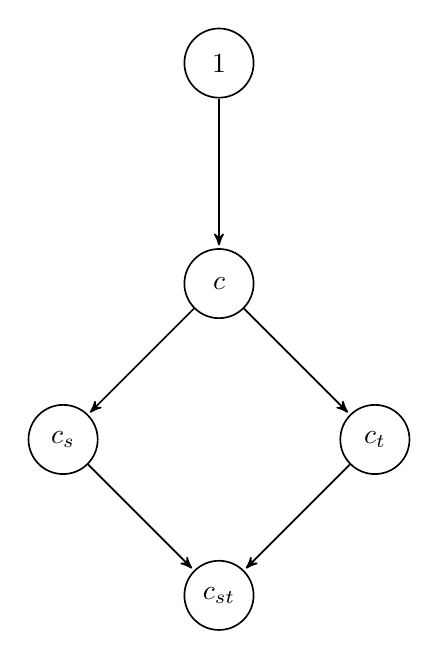
\begin{tikzpicture}[->,>=stealth',shorten >=1pt,auto,node distance=2.8cm, semithick]

    \node[state] (A)                    {$1$};
    \node[state] (B) [below of=A]       {$c$};
    \node[state] (C) [below left of=B]  {$c_s$};
    \node[state] (D) [below right of=B] {$c_t$};
    \node[state] (E) [below left of=D]  {$c_{st}$};

    \path       (A) edge node {} (B)
                (B) edge node {} (C)
                    edge node {} (D)
                (C) edge node {} (E)
                (D) edge node {} (E);
  \end{tikzpicture}
  
  \caption{Hierarchy of hypotheses.}
  \label{fig:hier}
\end{figure}

\subsection{Fully Observed Count Data}
\label{sec:count}

The likelihood function that allows for estimation of these parameters is as follows.  Since we assume $X_{jst}$ is independent of $Y_{ist}$ we can simply multiply the respective Poisson probability density functions, and then form products over all $s,t$ to get the likelihood.  

\begin{equation}
  \label{eq:likelihood}
  L(x_{jst}, y_{ist} |\boldsymbol{\lambda}, \boldsymbol{\gamma}) = \prod_{t = 1}^{T} \prod_{s=1}^S \left\{ \prod_{j=1}^{J_t} f_X(x_{jst}|\boldsymbol{\lambda}) \prod_{i=1}^{I_t} f_Y(y_{ist} | \boldsymbol{\gamma}) \right\}.
\end{equation}

\noindent Writing all five hypotheses as $\lambda_{st} = c_{st}\gamma_{st}$, we can, in the simplest cases, find analytic solutions for the maximum likelihood estimates of $c_{st}$ and $\gamma_{st}$.  Under the hypothesis $c_{st} = 1$, and when the data are balanced $J_t = J$, $I_t = I$, and $c_{st} = c$ analytic solutions exist.  Namely, these solutions are

\begin{equation*}
  \hat{\gamma}_{st} = \frac{X_{\cdot st} + Y_{\cdot st}}{J_t + I_t}, \quad \text{ and } \quad \hat{c} = \frac{I \sum_{s,t} X_{\cdot st}}{J \sum_{s,t} Y_{\cdot st}}, \quad \hat{\gamma}_{st} = \frac{X_{\cdot st} + Y_{\cdot st}}{I \left( \frac{\sum_{st} X_{\cdot st}}{\sum_{st} Y_{\cdot st}} + 1 \right)}
\end{equation*}

\noindent respectively, where $X_{\cdot st} = \sum_{j=1}^{J_t}X_{jst}$ and $Y_{\cdot st} = \sum_{i=1}^{I_t} Y_{ist}$.

In all other cases, analytic solutions are not readily available and instead we rely on the fact that the log-likelihood $l(\boldsymbol{\lambda}, \boldsymbol{\gamma}) = \log{L}$ is concave.  We maximize the log-likelihood, using coordinate descent \citep{Luo:1992}, by iteratively solving partial derivatives of $l$, with respect to $c_{st}$ and $\gamma_{st}$, set equal to zero

\begin{equation*}
  \hat{c} = \frac{\sum_{s,t} X_{\cdot st}}{\sum_t J_t \sum_s \gamma_{st}}, \quad \hat{c}_t =  \frac{\sum_s X_{\cdot st}}{J_t \sum_s \gamma_{st}}, \text{ or} \quad \hat{c}_s = \frac{\sum_{t}X_{\cdot st}}{\sum_t J_t \gamma_{st}}, \text{ and } \quad \hat{\gamma}_{st} = \frac{X_{\cdot st} + Y_{\cdot st}}{J_t c_{st} + I_t}.
\end{equation*}

\subsection{Unobserved Counts}
\label{sec:noncount}

% Working with biologists who study spider foraging, we have found that not all predators allow for easily counted prey species in their guts.  As an alternative strategy, we can rely on the DNA sequencing of a sample from the predators' guts.  If such sequencing returns a positive response, say a $1$ if a particular predator ate prey species $s$, and $0$ otherwise, we can, albeit with these incomplete data, model predators' eating preferences with the above framework using the EM algorithm.  

Many times it may not be possible to count the number of individuals of each prey species that are in a predator's gut.  Instead, it may only be possible to detect whether or not a predator consumed the prey species during a given period.  In this case we can still make inference about the predators' preferences for the different prey species by using the EM algorithm to compute maximum likelihood estimates. 

We denote the binary random variable indicating that the $j^{th}$ predator did in fact eat at least one individual of prey species $s$ in time period $t$ by $Z_{jst} = 1(X_{jst} > 0)$.  The variables are independent Bernoulli observations with success probability $p_{st} = P(Z_{jst}=1)= 1-\exp\{-\lambda_{st}\}$.  Despite not observing $X_{jst}$, we can compute maximum likelihood estimates of the parameters $\boldsymbol{\lambda}, \boldsymbol{\gamma}$ through the EM algorithm using the complete data log-likelihood
\[
l_{comp}(\boldsymbol{\lambda}, \boldsymbol{\gamma}) = \log f_{X,Y,Z}(\boldsymbol x, \boldsymbol y, \boldsymbol z|\boldsymbol{\lambda}, \boldsymbol{\gamma}) = \sum_{s=1}^{S} \sum_{t=1}^T \left[ \sum_{j=1}^{J_t} \log f_{X,Z}(x_{jst},z_{jst}|\boldsymbol{\lambda}) + \sum_{i=1}^{I_t}\log f_Y(y_{jst}|\boldsymbol{\gamma}) \right].
\]

The density of $Y_{jst}$ is exactly as in section~\ref{sec:count} and so we focus on deriving the joint density of $X_{jst}$ and $Z_{jst}$.  With the distribution of $Z_{jst}$ given above, we can compute $f_{X,Z}(x_{jst},z_{jst}|\boldsymbol{\lambda})$ by noting that $X_{jst}=0$ with probability 1 if $Z_{jst}=0$, and that $[X_{jst}|Z_{jst}=0]$ has a truncated Poisson distribution with density
\[
  f_{X|Y,Z,\boldsymbol{\lambda},\boldsymbol{\gamma}}(x_{jst}|z_{jst}) =
  \frac{\exp{\{-\lambda_{st}\}} \lambda_{st}^{x_{jst}}}{(1 - \exp{\{-\lambda_{st}\}}) x_{jst}!}1(x_{jst} > 0)
\]
and expected value
\[
\E_{X|Y,Z}X_{jst} = \frac{\lambda_{st} \exp{\{\lambda_{st} \}}}{\exp{\{ \lambda_{st} \}} - 1}.
\]
\noindent The joint density of $X_{jst}, Z_{jst}$ is then 
\begin{equation*}
    f_{X,Z|\boldsymbol{\lambda}}(x_{jst},z_{jst}) = \left\{
    \begin{array}{lr}
      \exp{\{ -\lambda_{st} \}}, & x_{jst}=0 \mbox{ and } z_{jst} = 0 \\
      \frac{\exp{\{-\lambda_{st} \}} \lambda_{st}^{x_{jst}}}{x_{jst}!}, & x_{jst} > 0 \mbox{ and } z_{jst} = 1 \\
      0 & \mbox{otherwise}
    \end{array}
  \right..
\end{equation*}

% introduce EM and its iterative steps earlier
% just a couple of general sentences; explain the two steps and what they do
% rubin and little (~1980); mclchalan and Krishnan book
% split up E and M step, with \cdot ^(k) notation earlier
% mention convergence criterion

The EM algorithm works by iterating two steps, the E-step and M-step, until the optimum is reached \citep{Dempster:1977,McLachlan:2007}.  Let $k$ index the iterations in the EM algorithm so that $\boldsymbol \lambda^{(k)}$ and $\boldsymbol \gamma^{(k)}$ denote the estimates computed on the $k^{th}$ M-step. The E-step consists of computing the expectation of $l_{comp}$ with respect to the conditional distribution of $X$ given the current estimates of the parameters
\[
Q^{(k)}(\boldsymbol{\lambda},\boldsymbol{\gamma}) = \E_{X|Y,Z,\boldsymbol{\lambda}^{(k)}} l_{comp}
\]
in order to remove the unobserved data. The M-step then involves maximizing $Q = \E l_{comp}$ with respect to the parameters in the model to obtain updated estimates of the parameters,
\[
(\boldsymbol{\lambda}^{(k+1)}, \boldsymbol{\gamma}^{(k+1)}) = \argmax_{(\boldsymbol{\lambda}, \boldsymbol{\gamma})} Q^{(k)}(\boldsymbol{\lambda}, \boldsymbol{\gamma}).
\]
These steps are then alternated until a convergence criterion monitoring subsequent differences in the parameter estimates/likelihood is met.  

The calculation of $Q^{(k)}(\boldsymbol{\lambda}, \boldsymbol{\gamma})$ is not difficult and is given by:
\begin{align}
  \label{eq:estep}
  \begin{split}
  Q^{(k)}(\boldsymbol{\lambda}, \boldsymbol{\gamma})
  & = \E \log{f_{X,Z|\boldsymbol{\lambda}}(X_{jst},z_{jst})} + \log{f_{Y|\boldsymbol{\gamma}}(y_{ist})} \\
  & = \sum_{s=1}^S \sum_{t=1}^T \sum_{j=1}^{J_t} \E \log{f_{X,Z|\boldsymbol{\lambda}}(X_{jst},z_{jst})}
  + \sum_{s=1}^S \sum_{t=1}^T \sum_{i=1}^{I_t} \log{f_{Y|\boldsymbol{\gamma}}(y)} \\
  & \propto \sum_{s,t,j} \left( - \lambda_{st} 
    + z_{jst} \log{\lambda_{st}} \E X_{jst} \right) + \sum_{s,t} \left( -I_t \gamma_{st} + Y_{\cdot st} \log{I_t \gamma_{st}} \right) \\
  & \propto \sum_{s,t} \left( -J_t \lambda_{st} + z_{\cdot st} \log{\lambda_{st}} \E (X_{jst}|\lambda_{st}^{(k)},\gamma_{st}^{(k)}) \right) + \sum_{s,t} \left( -I_t \gamma_{st} + Y_{\cdot st} \log{I_t \gamma_{st}} \right).
\end{split}
\end{align}
\noindent No analytic solution to the M-step exists, however, so we chose to maximize $Q$ with coordinate descent \citep{Luo:1992}.  In fact, as we only need find parameters that increase the value of $Q$ on each iteration, we forgo fully iterating to find the maximum and instead perform just one step uphill within each EM iteration.  Since $Q^{(k)}$ is concave and smooth in the parameters $\boldsymbol{\lambda}, \boldsymbol{\gamma}$, we are able to use the convergence of parameter estimates, $||(\boldsymbol{\lambda}^{(k)}, \boldsymbol{\gamma}^{(k)}) - (\boldsymbol{\lambda}^{(k+1)}, \boldsymbol{\gamma}^{(k+1)})||_{\infty} < \tau $, for some $\tau>0$, as our stopping criterion.

As we show in our simulation study, this generalized EM algorithm accurately estimates the parameters when values of $\lambda_{st}$ are relatively small, such that zeros are prevalent in the data $Z_{jst}$.  In this case, not too much information is lost since estimation of $\E Z_{jst}$ can be estimated well by the proportion of observed zeros.  On the other hand, if the predator consistently eats a given prey species, few to no zeros will show up in the observed data and $\E Z_{jst}$ is estimated to be nearly $1$.  The loss of information is best seen by attempting to solve for $\lambda_{st}$ in the equation $1 = \E Z_{jst} 1 - \exp\{-\lambda_{st}\}$.  As the proportion of ones in the observed data increases, we expect $\lambda_{st}$ to grow exponentially large.  When no zeros are present in the data, so that where only ones are observed, the likelihood can be made arbitrarily large by sending the parameter off to infinity.  

\subsection{Testing}

The likelihood ratio test statistic is

\begin{equation*}
  \label{eq:LRT}
    \Lambda(X,Y) := -2 \log{ \frac{ \sup_{\theta_0} L(\theta_0|X,Y)}{ \sup_{\theta_1} L(\theta_1|X,Y)} },
\end{equation*}

\noindent where $\theta_0, \theta_1$ represent the parameters estimated under the null and alternative hypotheses, respectively.  It is well known that the asymptotic distribution of $\Lambda$ is a $\chi_{\rho}^2$ distribution with $\rho$ degrees of freedom \citep{Wilks:1938}.  When the observations $X_{jst}$ are not observed, we use $L_{obs}(Z,Y)$ as the likelihood in the calculation of $\Lambda$.  

The degrees of freedom $\rho$ equal the number of free parameters available in the stated hypotheses under question.  If we put the null hypothesis to be $H_0: \lambda_t = c_t \gamma_t$, for all $t$ and contrast this against $H_1: \lambda_{st} = c_{st}\gamma_{st}$ then there are $\rho = 2(S \cdot T) - S \cdot T - T = S \cdot T - T$ degrees of freedom.

A set of hypotheses is determined by the p-value of the $\chi^2_{\rho}$ distribution.  Hence, with a level of significance, $\alpha$, the null hypothesis is rejected in favor of the alternative hypothesis if $\mathbb{P}(\chi^2_{\rho} > \Lambda) < \alpha$.  

\subsection{Linear Transformations of $c_{st}$}

After determining which model best fits the data, more detail can be extracted through a hypothesis test of the elements of $c_{st}$, or in vector notation as $\mathbf{c} \in \mathbb{R}^{S\cdot T}$.  Let the elements of $\hat{\mathbf{c}}$ be the maximum likelihood estimates, $\hat{c}_{st}$, as found via the framework above.  Since $\hat{\mathbf{c}}$ is asymptotically normally distributed, any linear combination of the elements is also asymptotically normally distributed.  For instance, let $a$ be a vector of the same dimension of $\hat{\mathbf{c}}$.  Then $a^t\hat{\mathbf{c}}$ is asymptotically distributed as $\mathcal{N}(a^t\mathbf{c}, a^t\Sigma a)$, where $\Sigma$ is the covariance matrix of the asymptotic distribution of $\hat{\mathbf{c}}$.  

Suppose, for example, that the hypothesis $c_s$ is determined to best fit the data with $s$ ranging $s = 1, 2, 3$.  We can test to see whether or not two species are statistically equally preferred under the null hypothesis $c_{1} = c_{2}$.  This hypothesis is alternatively written in vector notation as $a^t\mathbf{c} = 0$, where $a = (1, -1, 0)^t$.  Tests of the following form $H_0: a^t\mathbf{c} = \mu$ against any alternative of interest are then approximate $Z$-tests.  Confidence intervals of any size are similarly, readily obtained.  Of course, one could also use a $t$ distribution as a small sample size correction.

%%% Local Variables: 
%%% mode: latex
%%% TeX-master: "main"
%%% End: 

\section{Simulations}
\label{sec:sim}

% use language like: data generating model and fitted model, not hypotheses

Our simulations assume two prey species and five time points, throughout.  Of the hierarchy of hypotheses, we generate data under three models: $c, c_s, c_t$.  Sample sizes for both prey species and predator gut count observations are randomly chosen from four overlapping levels: ``small'' sample sizes are randomly sampled numbers in $[20,50]$, ``medium'' $[30,75]$, ``large'' $[50,150]$, and ``huge'' $[100,200]$.  This is repeated for each level of sample size.  We simulate $500$ replicate datasets for each of the twelve scenarios above for both types of data, fully observed count data, $X_{jst}$, and for non-count data, when we observe only a binary response, $Z_{jst} = 1(X_{jst}>0)$.  Each scenario is then fit with the true model that generated the data.  All simulations of non-count data use $\tau = 10^{-5}$ as the convergence tolerance.  A subset of the examples are provided here; the interested reader is referred to the supplementary materials for the complete simulation results.

For all simulated data, the true parameter values for the rate at which prey species are encountered in the wild are fixed to be $\gamma_{st} = \pi, \, \forall s,t$. The values of $\lambda_{st}$ are set with respect to each data generating model.  For model $c_{st} = c$, where predator preferences don't vary by either time or species, we put $\lambda_{st} = 2\pi, \forall s,t$.  Under model $c_s$, the ratio of rates vary by species only, so we put $\lambda_{1t} = \sqrt{2}$ and $\lambda_{2t} = \pi$.  Hence, $c_1 = \sqrt{2}/\pi \approx 0.45$ and $c_2 = 1$.  For the last model, $c_t$, the ratio of rates vary by time $t$.  Here, we put $\lambda_{st} = t$ for $t \in \{1, \ldots, 5 \}$.  

\begin{figure}
  \centering
  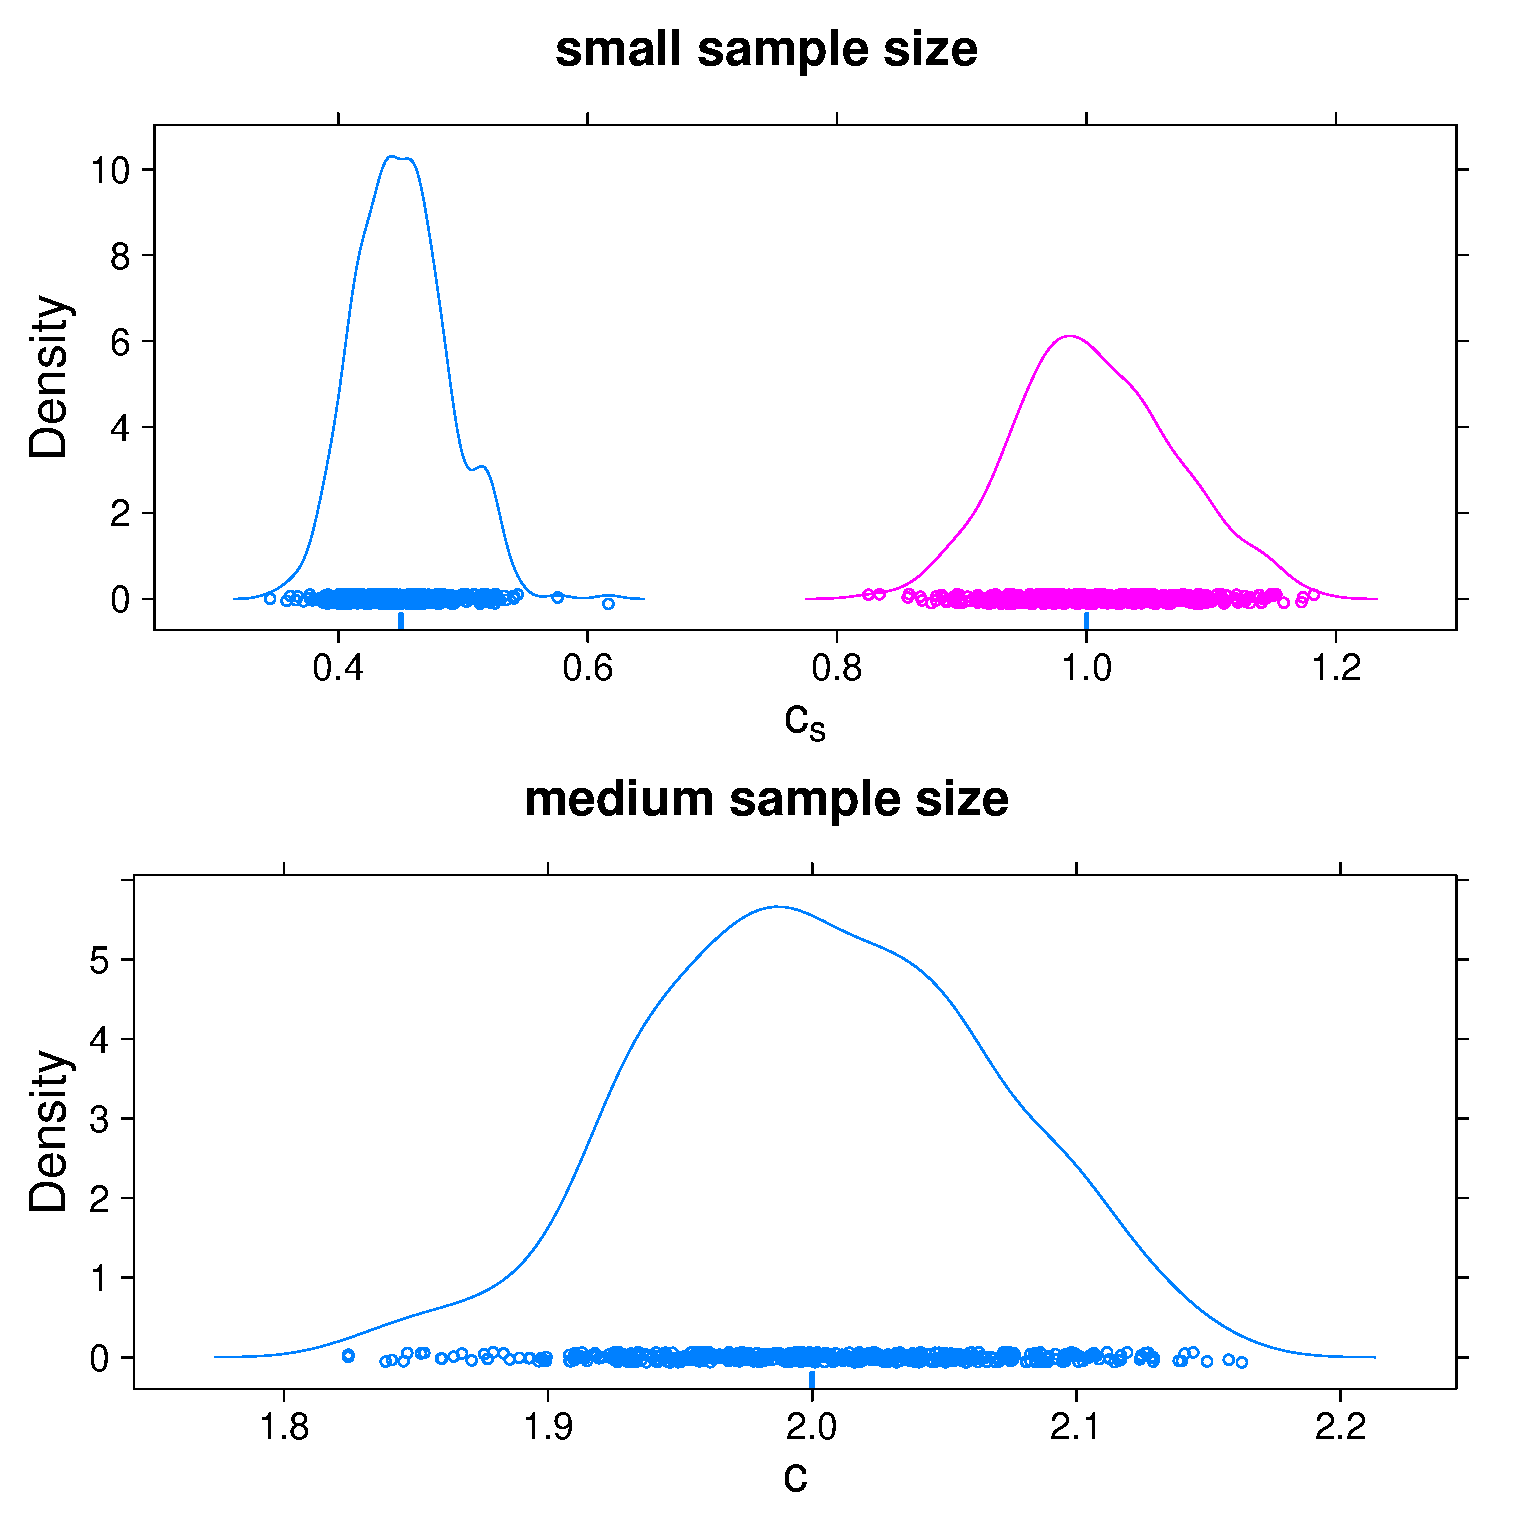
\includegraphics[scale=0.5]{nonem}
  \caption{Density plots of all $500$ estimates of fitting the true model to the data generated from models $c_s,c$ are shown with sample sizes small and medium, respectively.}
  \label{fig:nonem}
\end{figure}

% more words about how these numbers were estimated; estimtes from across all simulations
% simulations show nearly unbiased
% drop decimal places; we don't have precision to state further. 2

Figure~\ref{fig:nonem} shows density plots of the estimates of $c_s, c$ when fitting the true model to the fully observed count data generated under models $c_s$ and $c$.  The plots provide evaluations of parameter estimates under each scenario.  In the first display, the parameters $c_1 \approx 0.45$ and $c_2 = 1$ are on average, across all $500$ simulations, estimated as $\hat{c}_1 = 0.45$ and $\hat{c}_2 = 1.00$, with standard errors of $\text{se}(\hat{c}_1) = 0.03$ and $\text{se}(\hat{c}_2) = 0.06$.  The second display provides results for model $c_{st} = c$.  Averaging across all $500$ simulations, the parameter $c=2$ is estimated as $\hat{c} = 2.00$.  This is further seen in figure~\ref{fig:bp}, where box plots of the parameter estimates, centered at true parameter values, of the correct model fit to data generated from both $c_s$ and $c_t$ show empirically almost no bias.

\begin{figure}
  \centering
  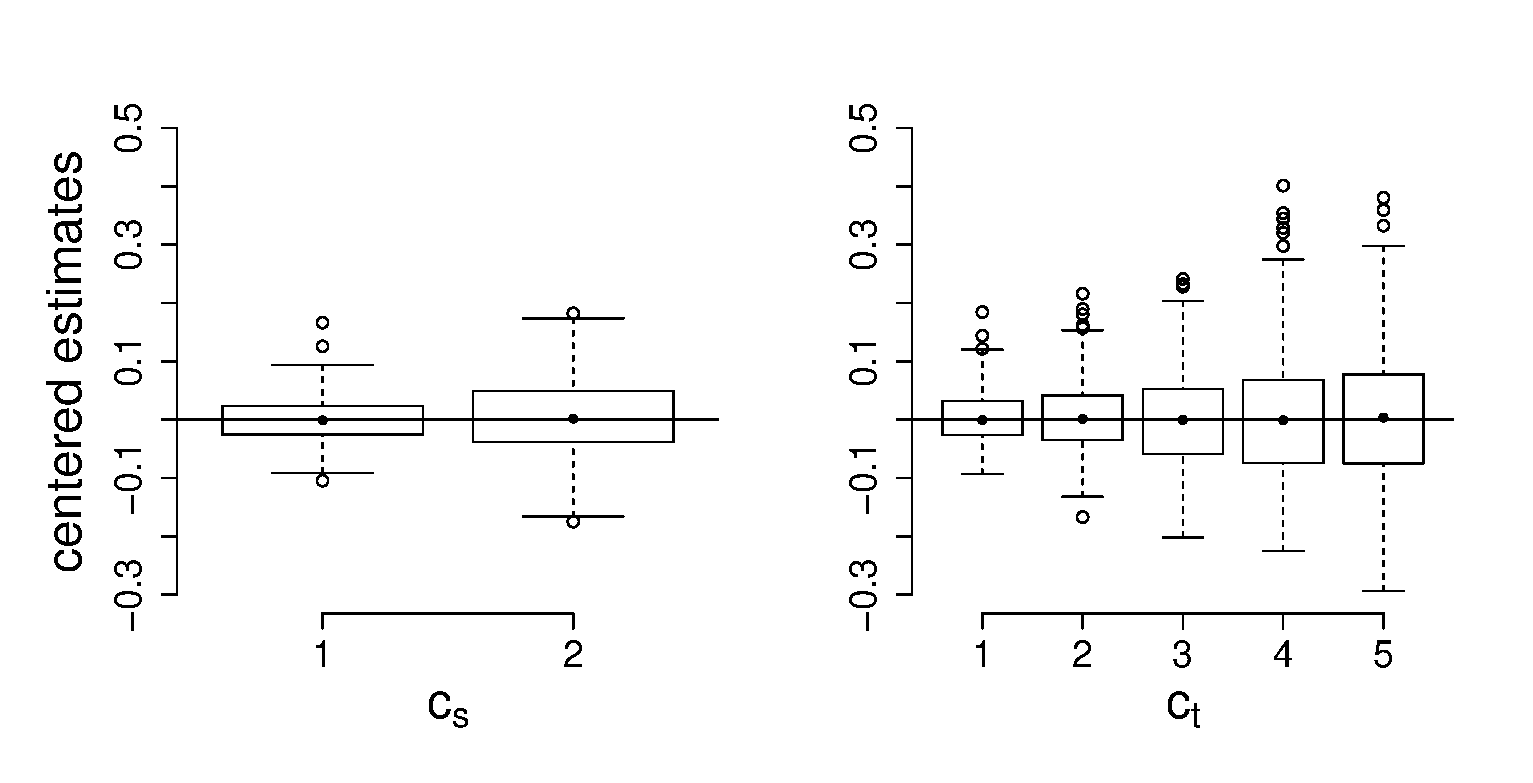
\includegraphics[scale=0.5]{bp}
  \caption{Shown are all $500$ estimates, centered at the true parameter values, from fitting the true model to the data generated from models $c_s,c$ with sample sizes small and medium, respectively.}
  \label{fig:bp}
\end{figure}

We next generated data with unobserved counts.  As noted above under certain circumstances our unobserved counts model accurately estimates the parameters of interest, and at different times can greatly over-estimate the parameters.  To investigate this issue further, we consider the same scenarios mentioned above, but now we reduce all of our count data down to binary observations.  For each scenario, we fit our unobserved counts model as if we knew the true underlying model that generated the observed data.

Figure~\ref{fig:em} contains density plots for all $500$ replications of the data generating models $c_s,c_t$ with small and huge sample sizes, respectively.  When data are generated under the model $c_s$ and the true model fit to the non-count data, we find even for the small sample size that point estimates are nearly unbiased.  When parameter values are of sufficient size to make zeros in the simulated data less common, the estimates from fitting the correct model to the generated data are occasionally over-estimated.  This effect is easily seen in the bottom panel of figure~\ref{fig:em} for larger values of $c_t$ despite the increased sample size, but is also seen, less dramatically, in the density plot for the $c_s$ generated data.  

{\color{red} Need to figure this out on computer then reconsider this paragraph.} The cluster of estimates for $c_5$ between $3.5$ and $4.0$ in the bottom panel of figure~\ref{fig:em} comes from datasets in which $X_{js5}>0$ so that $Z_{js5}>0$ for all $j$ and $s$. The probability that this happens is ? and we observed this in ? of the 500 data sets. As mentioned above, the estimate of $c_5$ is infinite in this case. However, the EM algorithm will always provide a finite estimate for all parameters when it terminates. In this case, we set $\tau=10^{-5}$ and it just happened that this caused the algorithm to terminate with $\hat c_5$ between 3.5 and 4.0 in all cases. To confirm that this is due to the arbitrary choice of $\tau$, we repeated the algorithm with smaller values of $\tau$ for several data sets. As expected, $\hat c_5$ increased without bound as we refit the model with smaller and smaller values of $\tau$.

% The seemingly arbitrary clustering of estimates near four seen in figure~\ref{fig:em} is caused by both the shape of the log-likelihood and the convergence tolerance, $\tau$.  As the proportion of ones in the $Z_{jst}$ observations increases, the observed log-likelihood becomes flatter.  Thus, any finite convergence tolerance will cause the algorithm to terminate eventually.  By decreasing $\tau$, and increasing, as appropriate, the maximum iterations allowed within the EM algorithm, one can gradually increase the magnitude of a maximum likelihood estimate.  For the tolerance we used in these simulations, $\tau = 10^{-5}$, four just happens to be where the algorithm stops.

% The plots of $\gamma_{st}$ under the EM algorithm are not given as we do not consider missing data in the estimation of these parameters. 

% more of which model are we fitting, which model is generating the data

\begin{figure}
  \centering
  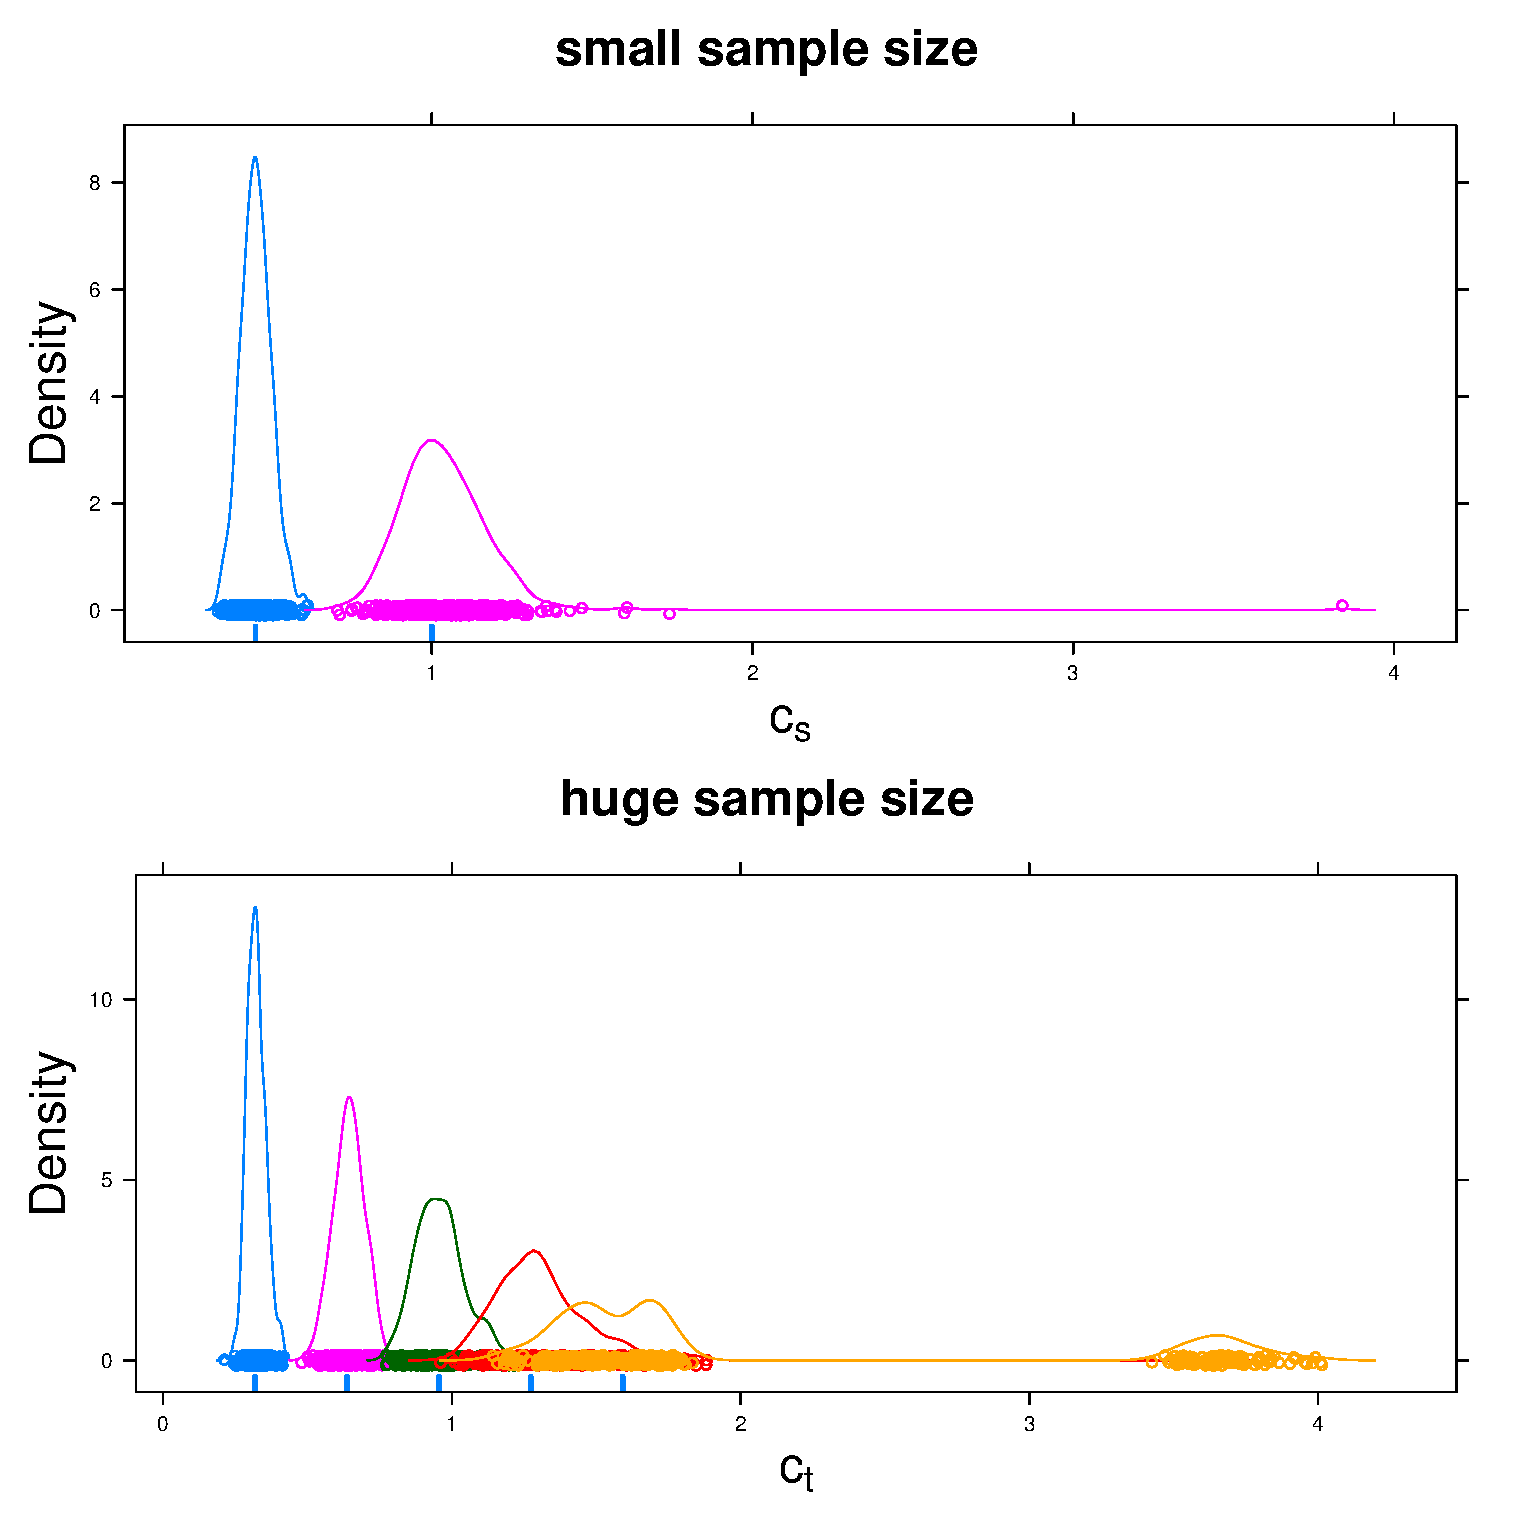
\includegraphics[scale=0.5]{em}
  \caption{Density plots of all $500$ estimates of fitting the true model to the data generated from models $c_s,c_t$, when counts are not observed, are shown with sample sizes small and huge, respectively.}
  \label{fig:em}
\end{figure}

{\color{red} Also address this paragraph after figuring out the computer issue.}  The over-estimation of parameters, a symptom of the loss of information due to the unobserved counts, can also be seen with box plots of the $500$ point estimates, centered at their respective true parameter values.  Figure~\ref{fig:em_bp} contains box plots of the same scenarios in Figure~\ref{fig:em}, but with the small and huge sample sizes.  It is clear that as the parameters values increase and zeros in the observed data $Z_{jst}$ become less prevalent, over-estimation occurs more frequently.  This over-estimation, when it occurs, will generally increase the magnitude of the bias.

%Table~\ref{tab:bias} displays the max absolute bias across all indices $s,t$ of $\lambda_{st}$ for each simulation scenario.


\begin{figure}
  \centering
  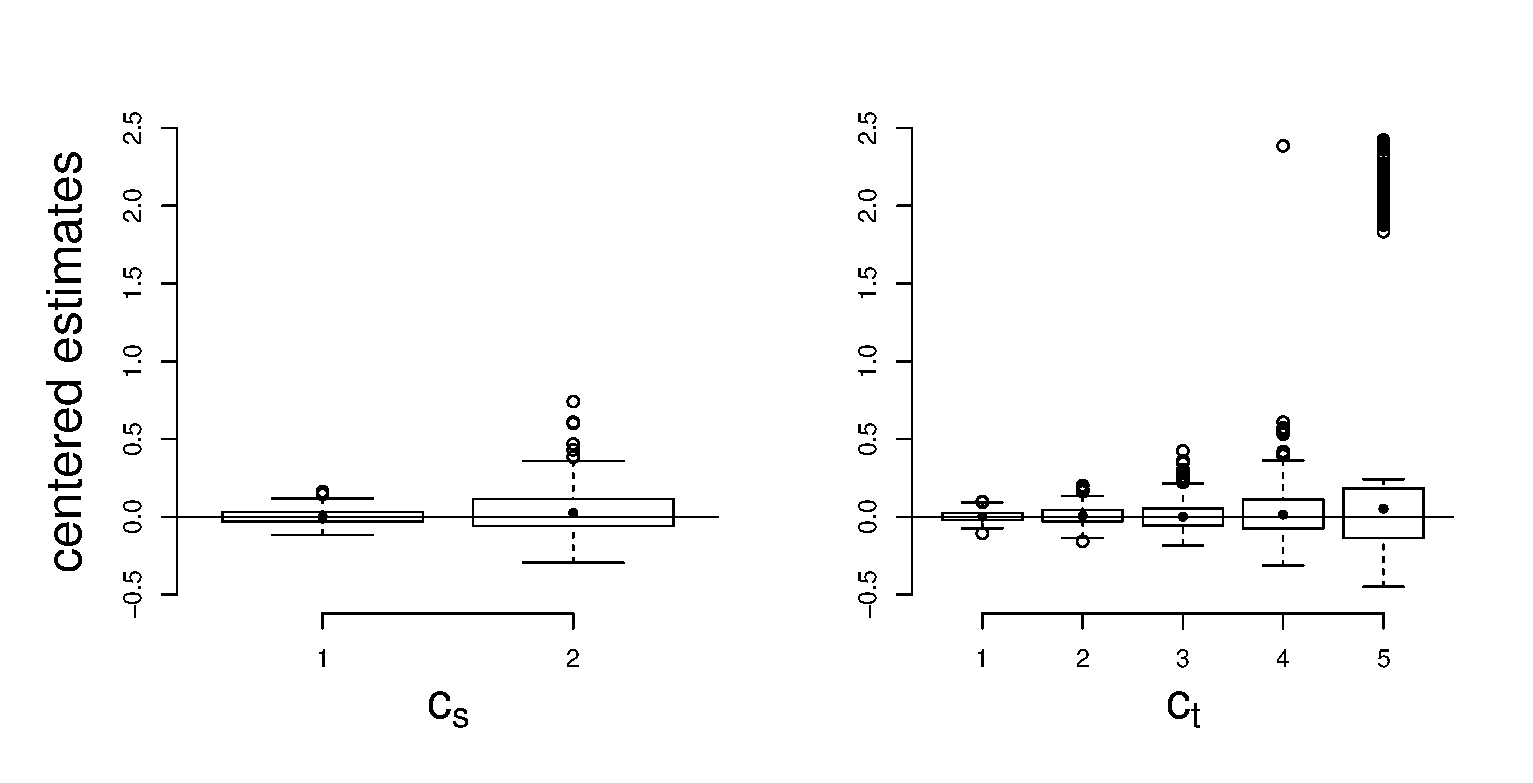
\includegraphics[scale=0.5]{em_bp}
  \caption{Shown are all $500$ estimates, centered at the true parameter values, from fitting the true model to the data generated from models $c_s,c_t$, when counts are not observed, with sample sizes small and huge, respectively.}
  \label{fig:em_bp}
\end{figure}

% \begin{table}
%   \centering
%   \begin{tabular}{ll|rrrr}
%     & & small & medium & large & huge \\ 
%     \hline
%     count & $c_t$ & 0.040 & 0.013 & 0.020 & 0.011 \\ 
%     & $c_s$ & 0.028 & 0.015 & 0.010 & 0.005 \\ 
%     & $c$ & 0.030 & 0.016 & 0.017 & 0.012 \\ 
%     non-count & $c_t$ & 4.151 & 3.155 & 0.941 & 1.423 \\ 
%     & $c_s$ & 0.138 & 0.096 & 0.044 & 0.032 \\ 
%     & $c$ & 2.924 & 2.078 & 0.669 & 0.547 \\ 
%   \end{tabular}
%   \caption{Max absolute bias of all $\lambda_{st}$ for each simulation scenario.}
%   \label{tab:bias}
% \end{table}

%%% Local Variables: 
%%% mode: latex
%%% TeX-master: "main"
%%% End: 

\section{Real Data}
\label{sec:data}

We use the dataset from {\color{red} our Biologist colleagues}, where interest lies in the Wolf spider, genus Schizocosa, and the prey orders Diptera, Collembola, for each month from October $2011$ to March $2013$.  Following our hierarchy of hypotheses, we find that the most parameter rich model, $\lambda_{st} = c_{st} \gamma_{st}$ where each month and each prey species is given its own parameter, fits these data best.  This estimates $72$ parameters in total, $32$ of which estimate $c_{st}$.

We demonstrate our method's ability to test linear constraints on $c_{st}$, by setting up a linear contrast that evaluates whether or not the model $c_t$ appropriately fits the data.  This linear contrast approach is the same as testing the null hypothesis $H_0: \lambda_{st} = c_t \gamma_{st}, \forall t$ against the alternative hypothesis $H_1: \lambda_{st} = c_{st} \gamma_{st}$, but with a different statistical test than the likelihood ratio test.  

To do this we use the thirty-six estimates of $c_{st}$ fit from our EM algorithm, together with the linear contrast, $a^t = (1, \ldots, 1, -1, \ldots, -1)^t$.  This linear contrast asks if a model with only one parameter for both prey orders within each time period fits as well as a model with two parameters for both prey orders in each time period.  Hence, the null hypothesis for this linear contrast is $H_0: a^tc_{st} = 0$ against the alternative hypothesis $H_1: a^tc_{st} \ne 0$.  The test gives $p-value < 2.2\times 10^{-16}$, indicating that the more parameter rich model is strongly favored, just as did the likelihood ratio test.


%%% Local Variables: 
%%% mode: latex
%%% TeX-master: "main"
%%% End: 

\section{Discussion}
\label{sec:discussion}

The model developed here allows predators' preferences by testing simultaneously across an array of multiple prey species and time points.  This is achieved via a simple, but statistically powerful, likelihood ratio test.  Further testing of the ratio of rates for which predators eat to encounter prey species allows researchers to make specific conclusions about predators' preferences.  For instance, rates across time can be estimated to make statements about seasonal effects on a predator's eating habits, or relative rates across species groups allows for statements about the relative preferences for different species.

When counts of predators' gut contents are not fully observed, and instead only a binary response indicating the existence of the prey species in the gut is observed, we are able to treat the counts as missing data.  By modeling all of the observed data, both the binary responses and the number of prey species caught, and the missing count data, we are able to use the EM algorithm to extract as much information from the data as possible.  Though this is nice in theory, in practice the success of this modification to our original model is limited by the magnitude of the unknown parameters $\lambda_{st}$.  

Further developments of our model could be beneficial.  Taking into account other environmental variables that might effect a predator's eating habits, such as rain or temperature might be advantageous.  

%%% Local Variables: 
%%% mode: latex
%%% TeX-master: "main"
%%% End: 

\section{Acknowledgments}
\label{sec:acknowledge}

The information reported in this paper (No. xx-xx-xxx) is part of a project of the Kentucky Agricultural Experiment Station and is published with the approval of the Director.  Support for this research was provided by the University of Kentucky Agricultural Experiment Station State Project KY008055 and the National Science Foundation Graduate Research Fellowship Program.

%%% Local Variables: 
%%% mode: latex
%%% TeX-master: "main"
%%% End: 

\section{Data Accessibility}
\label{sec:accessibility}

An \texttt{R} package, named \texttt{spiders}, is available on CRAN at \url{http://cran.r-project.org/web/packages/spiders/index.html} and fits all the methods discussed above.  

%%% Local Variables: 
%%% mode: latex
%%% TeX-master: "main"
%%% End: 


\bibliographystyle{plainnat}
\bibliography{refs}
\end{document}
